\documentclass[11pt, a4paper]{article}
\usepackage[T1]{fontenc}
\usepackage[a4paper, margin=2.5cm]{geometry}
\usepackage{tikz}
\usepackage{amsmath}
\usepackage{amsfonts}
\usepackage{amssymb}
\usepackage{mathtools}
\allowdisplaybreaks
\DeclareMathOperator{\GCD}{GCD}
\usepackage{listings}
\usepackage{parskip}
\usepackage{hyperref}
\hypersetup{
	colorlinks=true,
	linkcolor=blue,
	urlcolor=blue,
	citecolor=blue,
	pdftitle={A Rigorous Triadic Framework for Neurosymbolic Reasoning},
	pdfauthor={José Arturo Ornelas Brand}
}
\title{A Rigorous Triadic Framework for Neurosymbolic Reasoning}
\author{
	José Arturo Ornelas Brand \\
	\textit{Independent Researcher} \\
	\href{mailto:arturoornelas62@gmail.com}{\texttt{arturoornelas62@gmail.com}}
}
\date{\today}
\begin{document}
	\maketitle
	% --- ABSTRACT ---
	\begin{abstract}
		Current Large Language Models (LLMs) excel at statistical pattern matching but struggle with verifiable symbolic logic. This paper proposes a formal, integer-based relational framework as a candidate model for the underlying logic of emergent "sparse circuits" \cite{Anthropic_SparseCircuits}. The framework is built on \textbf{dual functions}: a \textit{generative} function ($\Phi_G$) for predicting new relations and a \textit{discovery} function ($\Phi_D$) for inferring balancing rules from existing data. It uses integer balancing and normalization via the Greatest Common Divisor (GCD) to compute relational transformations, moving beyond floating-point vector addition to a \textbf{ratio-based}, symbolic logic. We first define the formal mathematics. We then validate its descriptive power by modeling the laws of classical mechanics. Finally, we discuss its implementation in Python using exact rational arithmetic (\texttt{fractions}) and graph libraries (\texttt{networkx}) for building hybrid neurosymbolic architectures. We provide a Python implementation to validate the framework's computational viability.
	\end{abstract}
	% --- KEYWORDS ---
	\vspace{5mm}
	\noindent
	\textbf{Keywords:} Neurosymbolic AI, Relational Framework, Interpretability, Sparse Circuits, Knowledge Graphs, Greatest Common Divisor (GCD), Symbolic Reasoning, Rational Arithmetic, Automated Scientific Discovery, Hybrid Neurosymbolic Systems, Mechanistic Interpretability
	\tableofcontents
	\newpage
	% --- SECTION 1: INTRODUCTION ---
	\section{Introduction: The Need for a Symbolic Logic in AI}
	The field of Artificial Intelligence has been revolutionized by Large Language Models (LLMs). Their ability to perform analogical reasoning, such as the famous $\vec{\text{King}} - \vec{\text{Man}} + \vec{\text{Woman}} \approx \vec{\text{Queen}}$ operation \cite{Mikolov2013}, is a product of high-dimensional vector arithmetic in a continuous, floating-point space. While powerful, this \textit{additive} approach lacks the rigorous, verifiable, and discrete logic required for many scientific domains.
	Recent research on "sparse circuits" \cite{Anthropic_SparseCircuits} suggests that LLMs implicitly learn functional subgraphs. However, a formal language to describe the \textit{logic} of these circuits is missing. We are left with statistical correlations rather than explainable computations.
	This paper proposes a candidate for this formal language: a \textbf{Triadic Relational Framework} based on normalized integers. We move from an additive relationship ($A - B + C = D$) to a \textbf{ratio-based} one ($\Phi(A, B, C) \rightarrow D$) grounded in integer balancing and the Greatest Common Divisor (GCD).
	We will first present the formal mathematics. We will then demonstrate its applicability with two case studies:
	\begin{enumerate}
		\item \textbf{Classical Mechanics:} Modeling the deterministic, formula-based laws of physics as a hierarchical graph.
		\item \textbf{AI Interpretability:} Proposing this framework as a formal model for sparse circuits and neurosymbolic systems, including a novel semantic mapping scheme (as detailed in Sec. 4.4).
	\end{enumerate}
	% --- SECTION 2: THE FORMAL TRIADIC FRAMEWORK ---
	\section{A Formal Triadic Relational Framework}
	This model is generalized into a formal mathematical framework which uses integer-based normalization to describe relational triads, designed to unify physical and abstract concepts.
	% --- SUBSECTION 2.1 ---
	\subsection{The Dual Functions of the Framework}
	The framework is built upon two complementary functions: a Generative function ($\Phi_G$) for prediction, and a Discovery function ($\Phi_D$) for inference.
	\subsubsection{Generative Function (\texorpdfstring{$\Phi_G$}{Phi-G}): The 4-Step Process}
	The $\Phi_G$ function predicts a new concept $C_4$ from three inputs $(C_1, C_2, C_3)$ and a known rule $(a, b)$. This is a 4-step process:
	\begin{enumerate}
		\item \textbf{Input Concepts:} We start with three known concepts (inputs): $C_1, C_2, C_3$.
		\item \textbf{Normalization:} We compute a common divisor for the inputs: $\GCD_{\text{in}} = \GCD(C_1, C_2, C_3)$. We then normalize the inputs to their integer base: $C_i' = C_i / \GCD_{\text{in}}$.
		\item \textbf{Relational Transformation:} A triadic relation $\Phi_G$ is applied. This relation is defined by a pair of minimal, co-prime integers ($a, b \in \mathbb{Z}^+$) that represent the "rule" of the triad. The transformation predicts a normalized output, $C_4'$.
		\[
		\Phi_G(C_1', C_2', C_3') \rightarrow C_4' \quad \text{where} \quad C_4' = \frac{a \cdot C_2' \cdot C_3'}{b \cdot C_1'}
		\]
		This is derived from the balancing equation: $a \cdot C_2' \cdot C_3' = b \cdot C_1' \cdot C_4'$. Other $\Phi$ functions are also possible (see Sec 4.3).
		\item \textbf{Denormalization:} The final, concrete output $C_4$ is retrieved by scaling the normalized output by the input divisor: $C_4 = C_4' \cdot \GCD_{\text{in}}$. The computation must result in an integer $C_4$, or the relation is considered invalid for this rule.
	\end{enumerate}
	\subsubsection{Discovery Function (\texorpdfstring{$\Phi_D$}{Phi-D}): Inferring Rules}
	Alongside the generative function, the framework includes a crucial \textbf{Discovery Function ($\Phi_D$)}. This function operates in reverse: given a known, balanced set of four concepts $(C_1, C_2, C_3, C_4)$, it infers the minimal, co-prime balancing coefficients $(a, b)$ and the associated simplicity $K$.
	\[
	\Phi_D(C_1, C_2, C_3, C_4) \rightarrow (a, b, K)
	\]
	This is achieved by first normalizing all four inputs by their GCD ($\GCD_{\text{in}} = \GCD(C_1, C_2, C_3, C_4)$), and then computing the exact rational ratio $\frac{a}{b}$, which is simplified to its minimal co-prime form:
	\[
	\frac{a}{b} = \frac{C_1' \cdot C_4'}{C_2' \cdot C_3'}
	\]
	The simplicity is then $K = 1 / (a \cdot b)$. This function is essential for analyzing existing data and discovering the underlying rules of a system (see Sec 3.2). Note that the assignment of roles (e.g., which concept is $C_1$ vs. $C_2$) is a crucial modeling step, as it determines the sides of the balance equation. This assignment is typically performed by the researcher or, in a neurosymbolic system, learned by the neural component (see Sec 4.4).
	\subsection{Key Components of the Framework}
	The framework separates the logic into node-level computations and network-level connections for clarity:
	\begin{itemize}
		\item \textbf{Node Logic (Triad $\Delta$):} The simplest stable unit is a triad $\Delta(C_1, C_2, C_3; K)$, where the relational mechanism $\Phi$ (e.g., $\Phi_G$ or $\Phi_D$) computes the output $C_4'$ from normalized inputs $C_i'$ using co-prime $a, b$. The triad is quantified by a simplicity constant \textbf{$K = 1 / (a \cdot b)$}. This metric measures the simplicity of the rule: higher $K$ indicates simpler rules (e.g., $a=1, b=1$ yields $K=1$, the maximum simplicity). Normalized $C_i'$ bridge physical and abstract domains.
		\item \textbf{Network Logic ($\mathcal{N}$):} Triads connect to form graphs. The output $C_4$ of one triad seeds new triads, modeling dynamic systems. Connectivity is defined by $\mathcal{N}(\Delta_i, \Delta_j) = w_{ij} \cdot A_{ij}$, where $A_{ij}$ is the adjacency matrix (1 if $C_4$ from $\Delta_i$ inputs to $\Delta_j$, 0 otherwise), and $w_{ij} = K_i$ (the simplicity of $\Delta_i$) prioritizes paths with fundamental rules.
	\end{itemize}
	% --- SUBSECTION 2.3 ---
	\subsection{Chaining Triads and Networks}
	The network logic enables chaining: The output of one triad, $C_4$, can serve as an input for a new triad, $\Delta_2(C_4, C_5, C_6) \rightarrow C_7$. This forms a chain or graph.
	This is implemented as a \textbf{directed graph} (using \texttt{networkx}), where each node $\Delta_i$ stores its simplicity $K_i$.
	For example, if $\Delta_1(18, 6, 8) \rightarrow C_4=2$ (from Sec. 2.4), its output $C_4=2$ can feed $\Delta_2$:
	\begin{itemize}
		\item Let $\Delta_2$ be $\Delta_2(C_4=2, C_5=5, C_6=10) \rightarrow C_7$.
		\item Assume $\Delta_2$ has a simple rule $a=1, b=1$ ($K_2=1$).
		\item $\GCD_{\text{in}} = \GCD(2, 5, 10) = 1$. So $C_i' = C_i$.
		\item $C_7' = \Phi_G(2, 5, 10) = \frac{1 \cdot 5 \cdot 10}{1 \cdot 2} = 25$.
		\item $C_7 = C_7' \cdot 1 = 25$.
		\item This creates a chain $\Delta_1 \to \Delta_2$ producing a final output of 25. The edge $\Delta_1 \to \Delta_2$ would have weight $w_{12} = K_1 = 1/12$.
	\end{itemize}
	\subsection{Abstract Numerical Example (Using \texorpdfstring{$\Phi_G$}{Phi-G})}
	Consider an abstract system with three inputs: $C_1 = 18$, $C_2 = 6$, $C_3 = 8$. We wish to apply a rule defined by $a=3, b=4$.
	\begin{enumerate}
		\item \textbf{Input Concepts}: $C_1 = 18$, $C_2 = 6$, $C_3 = 8$.
		\item \textbf{Normalize}: $\GCD_{\text{in}} = \GCD(18, 6, 8) = 2$.
		\begin{itemize}
			\item $C_1' = 18 / 2 = 9$
			\item $C_2' = 6 / 2 = 3$
			\item $C_3' = 8 / 2 = 4$
		\end{itemize}
		\item \textbf{Apply $\Phi_G$}: We apply the rule $a=3, b=4$.
		\[
		C_4' = \frac{a \cdot C_2' \cdot C_3'}{b \cdot C_1'} = \frac{3 \cdot 3 \cdot 4}{4 \cdot 9} = \frac{36}{36} = 1
		\]
		\item \textbf{Denormalize (Revert)}:
		\[
		C_4 = C_4' \cdot \GCD_{\text{in}} = 1 \cdot 2 = 2
		\]
	\end{enumerate}
	Thus, the triad $(18, 6, 8)$ transforms into $2$. The simplicity of this rule is $K = 1 / (3 \cdot 4) = 1/12$.
	% --- SECTION 3: CASE STUDY 1 (PHYSICS) ---
	\section{Case Study 1: Modeling Classical Mechanics}
	To demonstrate the framework's descriptive power, we apply it to the concepts of classical mechanics.
	\subsection{Core Concepts as a $K_3$ Graph}
	We define three pillars of classical mechanics as a foundational graph: \textbf{Newton's Laws of Motion}, \textbf{Kinetic/Potential Energy}, and \textbf{Gravity/Acceleration}. In graph theory, this is a complete graph $K_3$.
	\begin{itemize}
		\item \textbf{Vertex A:} Newton's Laws of Motion
		\item \textbf{Vertex B:} Kinetic and Potential Energy
		\item \textbf{Vertex C:} Gravity and Acceleration
	\end{itemize}
	The three edges illustrate the interrelationships:
	\begin{enumerate}
		\item \textbf{Edge A$\leftrightarrow$B (Laws $\leftrightarrow$ Energy):} The work-energy theorem.
		\item \textbf{Edge B$\leftrightarrow$C (Energy $\leftrightarrow$ Gravity):} Gravity (acceleration $g$) defines potential energy ($PE = mgh$).
		\item \textbf{Edge C$\leftrightarrow$A (Gravity $\leftrightarrow$ Laws):} Gravity is a force, described by Newton's 2nd Law ($F_g = mg$).
	\end{enumerate}
	\begin{figure}[htbp]
		\centering
		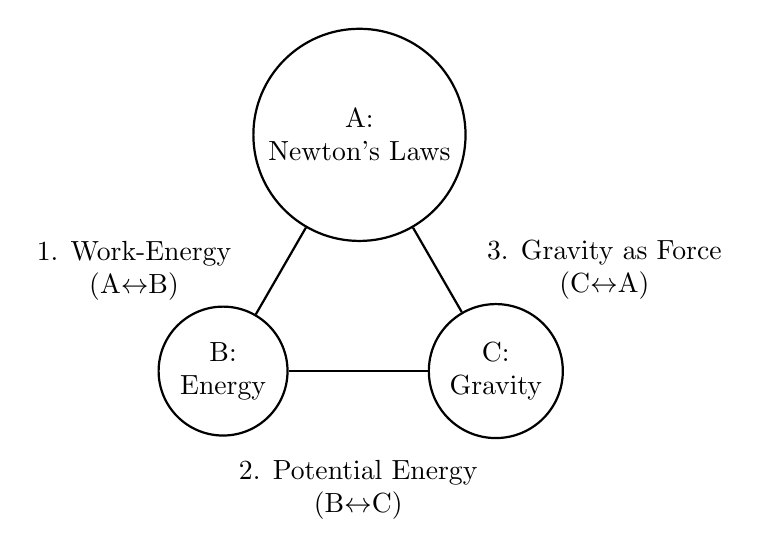
\begin{tikzpicture}[node distance=2.5cm, auto, thick]
			\node (A) at (90:2) [draw, circle, minimum size=1.5cm, align=center] {A: \\ Newton's Laws};
			\node (B) at (210:2) [draw, circle, minimum size=1.5cm, align=center] {B: \\ Energy};
			\node (C) at (330:2) [draw, circle, minimum size=1.5cm, align=center] {C: \\ Gravity};
			\draw (A) -- (B) node[midway, left, align=center, xshift=-5mm] {1. Work-Energy \\ (A$\leftrightarrow$B)};
			\draw (B) -- (C) node[midway, below, align=center, yshift=-10mm] {2. Potential Energy \\ (B$\leftrightarrow$C)};
			\draw (C) -- (A) node[midway, right, align=center, xshift=5mm] {3. Gravity as Force \\ (C$\leftrightarrow$A)};
		\end{tikzpicture}
		\caption{A $K_3$ complete graph showing the interrelationship between the three pillars of classical mechanics.}
		\label{fig:physics_graph}
	\end{figure}
	% --- SUBSECTION 3.2 ---
	\subsection{Handling Physical Formulas and Coefficients}
	The framework's balancing coefficients ($a, b$) are ideal for handling physical formulas. Instead of manually mapping them, we use the \textbf{Discovery Function ($\Phi_D$)} defined in Sec 2.1.2.
	For example, to analyze Kinetic Energy ($KE = \frac{1}{2}mv^2$, which is rewritten as $2 \cdot KE = 1 \cdot m \cdot v^2$), we analyze a known balanced set of concepts. Our framework's balance equation is $b C_1' C_4' = a C_2' C_3'$. To map the physics equation, we assign roles as follows: $C_1=KE$, $C_2=m$, $C_3=v^2$, and introduce a unit concept $C_4=1$ as a placeholder to complete the triad. This assignment implies $b \cdot KE \cdot 1 = a \cdot m \cdot v^2$, and we expect $\Phi_D$ to discover $a=1$ and $b=2$. Note that this role assignment is a crucial modeling step, determined by the structure of the formula (e.g., isolating the "output" or balancing sides).
	We test this with integer values that satisfy the relation, **matching those in our Appendix test code**: $KE=1, m=1, v= \sqrt{2} \rightarrow v^2=2$:
	\begin{itemize}
		\item We apply $\Phi_D(C_1=1, C_2=1, C_3=2, C_4=1)$.
		\item $\GCD_{\text{in}} = \GCD(1, 1, 2, 1) = 1$. All $C_i' = C_i$.
		\item The function computes the ratio based on the formal definition in Sec 2.1.2:
		\[
		\frac{a}{b} = \frac{C_1' \cdot C_4'}{C_2' \cdot C_3'} = \frac{1 \cdot 1}{1 \cdot 2} = \frac{1}{2}
		\]
		\item It thus *discovers* the minimal balancing coefficients $a=1, b=2$, correctly matching the $2 \cdot KE = 1 \cdot m \cdot v^2$ formulation.
	\end{itemize}
	For formulas with irrational constants (e.g., $C = 2\pi r$), the framework can operate on integer-scaled approximations. We can approximate $\pi \approx 22/7$, leading to $7C \approx 44r$. We map this as $bC = ar$ (using $C_1=C, C_2=r, C_3=1, C_4=1$). Using $\Phi_D$ on known values $C_1=44, C_2=7, C_3=1, C_4=1$, it discovers the ratio:
	\[
	\frac{a}{b} = \frac{C_1' \cdot C_4'}{C_2' \cdot C_3'} = \frac{44 \cdot 1}{7 \cdot 1} = \frac{44}{7}
	\]
	This yields $a=44, b=7$, successfully discovering the integer-approximated rule.
	As a simpler example, Ohm's Law ($V = IR$) maps to a direct $a=1, b=1$ rule. By assigning roles $C_1=V, C_2=I, C_3=R, C_4=1$ and testing known integer values (e.g., $V=10, I=2, R=5$), $\Phi_D$ correctly discovers the simplest ratio $\frac{a}{b} = \frac{10 \cdot 1}{2 \cdot 5} = \frac{1}{1}$, yielding $a=1, b=1$ and the maximum simplicity $K=1$.
	% --- SECTION 4: CASE STUDY 2 (AI) ---
	\section{Case Study 2: A Model for AI Interpretability}
	The triadic framework, demonstrated with physics, proposes a general-purpose model for relational logic. This formalism has profound implications for Artificial Intelligence, particularly in the growing field of neurosymbolic systems \cite{Garcez2023}.
	\subsection{Formalizing Sparse Circuits}
	A primary challenge in AI interpretability is understanding the \textit{logic} of emergent "sparse circuits" \cite{Anthropic_SparseCircuits}. The framework proposed here offers a candidate model for formally describing this logic.
	\begin{itemize}
		\item Our model provides a path to move from a \textbf{statistical correlation} (the LLM's "black box") to an \textbf{explicit logical computation} (the $\Phi$ function with GCD normalization).
	\end{itemize}
	In essence, while LLMs find \textit{what} concepts are related, our model offers a language to describe \textit{how} and \textit{why} they are related. This discrete approach could also reduce hallucinations in LLMs by enforcing verifiable, logical balances.
	\subsection{Integer-Based Relations vs. Vector Additivity}
	As noted, LLMs use analogical reasoning via vector arithmetic. This is an \textbf{additive} relationship. Our model proposes a \textbf{ratio-based} relationship defined by integers ($a, b$). This approach may offer a more stable and generalizable method for capturing symbolic analogies.
	\subsection{Formalizing the "King-Queen" Analogy}
	Let's contrast the two models for the famous analogy.
	\begin{itemize}
		\item \textbf{Vector (Additive) Model:}
		\[
		\vec{\text{King}} - \vec{\text{Man}} + \vec{\text{Woman}} \approx \vec{\text{Queen}}
		\]
		This is a statistical approximation in a continuous vector space.
		\item \textbf{Triadic (Ratio-Based) Model:}
		The standard "A is to B as C is to D" analogy ($C_1:C_2 :: C_3:C_4$) is a ratio-based operation: $\frac{C_1}{C_2} = \frac{C_3}{C_4}$. This implies a generative function $\Phi_A$ (for Analogy):
		\[
		\Phi_A(C_1, C_2, C_3) \rightarrow C_4 \quad \text{where} \quad C_4 = \frac{C_1 \cdot C_3}{C_2}
		\]
		This is a variant of our framework's $\Phi_G$ function (one where the inputs are arranged differently and $a=1, b=1$). Let's test this symbolic, integer-based math.
	\end{itemize}
	\subsection{Mapping Semantic Concepts to Integers}
	A critical challenge is mapping abstract concepts like "King" to the integers $C_i$ required by our framework. This mapping is the key "neural" component of a neurosymbolic system, where a model learns a function $f(\text{concept}) \rightarrow \mathbb{Z}$ based on latent factors (e.g., prime decompositions for orthogonal attributes). The success of our framework hinges on this learned representation: the neural layer must produce integers that enable balanced, simple triads (integer $C_4$ with high $K$).
	
	To demonstrate feasibility, consider a simple scheme where attributes are mapped to primes (assuming orthogonality; in practice, a neural layer would learn these):
	\begin{itemize}
		\item Attribute(Royalty) = 7
		\item Attribute(Male) = 3
		\item Attribute(Female) = 5
	\end{itemize}
	Concepts are products:
	\begin{itemize}
		\item $C_1 (\text{King}) = 7 \cdot 3 = 21$
		\item $C_2 (\text{Man}) = 3$
		\item $C_3 (\text{Woman}) = 5$
	\end{itemize}
	Applying $\Phi_A$: ($\GCD(21, 3, 5) = 1$)
	\[
	C_4 = \frac{21 \cdot 5}{3} = 35 = 7 \cdot 5 (\text{Queen})
	\]
	This integer-based calculation succeeds. In a full system, the neural model could be trained with our framework as a loss function: minimize loss when predicted integers yield integer balances with high $K$.
	% --- SECTION 5: CONCLUSION AND FUTURE WORK ---
	\section{Conclusion and Future Work}
	This paper has introduced a formal triadic relational framework based on integer balancing and GCD normalization. We have demonstrated its utility by modeling the deterministic laws of classical physics and by proposing it as a formal language for AI interpretability, built upon dual generative ($\Phi_G$) and discovery ($\Phi_D$) functions.
	This convergence of the neural and symbolic layers forms our primary path for future work. The initial goal of discovering new physical relationships from a complete "graph of physics," (as outlined in \cite{arXiv_PhysicsGraph}) is computationally intractable to build manually.
	However, we propose using the \textbf{Neural Layer (LLM)} as an advanced mining tool to parse scientific literature and automatically extract the knowledge graph and candidate triads ($C_1, C_2, C_3$). More crucially, the LLM can learn the mapping $f(\text{concept}) \rightarrow \mathbb{Z}$, producing integer representations that enable balanced triads. The \textbf{Symbolic Layer (our $\Phi$ Framework)} will then analyze these triads. By using $\Phi_D$ to find triads with simple rules (high $K$ value), our framework can act as a generative engine (using $\Phi_G$) to predict new, verifiable formulas ($C_4$). This framework provides an ideal loss function for training the neural mapper: reward mappings that yield integer $C_4$ with high $K$, moving beyond simple analogy to true automated scientific discovery.
	\textbf{Limitations and Implementation:} A reference implementation of this framework has been developed in Python. It utilizes \texttt{math.gcd} for normalization, the \texttt{fractions} library to ensure exact rational arithmetic (eliminating floating-point errors in $K$), and \texttt{networkx} to construct and manage the relational knowledge graphs. This implementation confirms the computational viability of the dual $\Phi_G$ and $\Phi_D$ functions.
	Future work will focus on extending this deterministic, ratio-based model. This modularity can be achieved without altering the core logic. For instance, **probabilistic** relationships can be modeled by introducing distributions (e.g., via Monte Carlo sampling on $a$ and $b$) to handle uncertainty. Similarly, **additive** relationships (common in LLM vector analogies) can be integrated by defining a hybrid $\Phi$ function (e.g., $\Phi_H = \Phi_G + \Phi_{Additive}$) that combines ratio-based and additive operations, bridging the gap to modern neural architectures. Further research will also investigate the framework's scalability, using efficient graph algorithms to manage networks of thousands of triads. We aim to implement a neurosymbolic prototype that utilizes this framework's balancing rules as a loss function for training on relational datasets, such as those found in standard analogy benchmarks.
	
	
	% --- SECTION 6: ACKNOWLEDGMENTS ---
	\section*{Acknowledgments}
	AI tools were employed for auxiliary tasks such as assistance in the LaTeX formatting, Python code debugging, and iterative refinement of the prose in this manuscript. The core concepts, framework logic, and final conclusions remain the original work of the author.
	

	% --- BIBLIOGRAPHY SECTION ---
	\newpage
	\begin{thebibliography}{9}
		\bibitem{Anthropic_SparseCircuits}
		Marks, S., Rager, C., Michaud, E. J., Veličković, P., Yacoby, Y., Kravec, S., Laidlaw, C., Aitchison,M., Prabakaran, S., McCaffrey, R., Graham, L., Duong, D. H., Perez, E., Bengio, Y., and Tegmark, M. (2024).
		Sparse Feature Circuits: Discovering and Editing Interpretable Causal Graphs in Language Models
		\textit{arXiv preprint arXiv:2403.19647}.
		\bibitem{arXiv_PhysicsGraph}
		Romiti, M. (2025).
		A Graph-Based Framework for Exploring Mathematical Patterns in Physics: A Proof of Concept.
		\textit{arXiv preprint arXiv:2508.05724}.
		\url{https://arxiv.org/abs/2508.05724}.
		\bibitem{Mikolov2013}
		Mikolov, T., Chen, K., Corrado, G., \& Dean, J. (2013).
		Efficient Estimation of Word Representations in Vector Space.
		\textit{arXiv preprint arXiv:1301.3781}.
		\bibitem{Garcez2023}
		Garcez, A. d'A., \& Lamb, L. C. (2023).
		Neurosymbolic AI: the 3rd wave.
		\textit{Artificial Intelligence Review, 56(11):12387-12406}.
	\end{thebibliography}
	% --- APPENDIX ---
	\newpage
	\appendix
	\section{Appendix: Core Python Implementation}
	This section contains the core Python code for the framework, demonstrating the implementation of the `TriadicRelationalFramework` (with its dual functions) and the `TriadicNetwork` class.
	\begin{lstlisting}[
		language=Python,
		basicstyle=\ttfamily\small,
		breaklines=true,
		frame=tb,
		caption={Core Python Implementation},
		label={lst:code},
		keepspaces=true 
		]
import math
from fractions import Fraction
import networkx as nx

class TriadicRelationalFramework:
	def __init__(self):
		pass # No initial state needed for basic implementation

	def compute_triad(self, C1, C2, C3, a, b):
		"""
		Compute the triadic relational transformation.

		Parameters:
		- C1, C2, C3: Input integer concepts
		- a, b: Positive integer balancing coefficients (minimal, co-prime)

		Returns:
		- C4: The computed output integer
		- K: The simplicity constant (Fraction: 1 / (a * b))
		- steps: Dictionary with intermediate steps for transparency
		"""
		if not all(isinstance(x, int) and x > 0 for x in [C1, C2, C3, a, b]):
			raise ValueError("All inputs must be positive integers.")

		steps = {}

		# Step 1: Input Concepts
		steps['inputs'] = {'C1': C1, 'C2': C2, 'C3': C3, 'a': a, 'b': b}

		# Step 2: Normalization
		gcd_in = math.gcd(C1, C2, C3)
		C1_prime = C1 // gcd_in
		C2_prime = C2 // gcd_in
		C3_prime = C3 // gcd_in
		steps['normalization'] = {'gcd_in': gcd_in, 'C1_prime': C1_prime, 'C2_prime': C2_prime, 'C3_prime': C3_prime}

		# Step 3: Relational Transformation (Phi)
		numerator = a * C2_prime * C3_prime
		denominator = b * C1_prime
		C4_prime = Fraction(numerator, denominator)
		steps['transformation'] = {'C4_prime': str(C4_prime)}

		# Step 4: Denormalization
		C4 = C4_prime * gcd_in
		if C4.denominator != 1:
			raise ValueError("The balancing does not result in an integer C4_prime. Adjust a, b or inputs.")
		C4 = int(C4) # Convert to int if integer
		steps['denormalization'] = {'C4': C4}

		# Simplicity K
		K = Fraction(1, a * b)
		steps['K'] = str(K)

		return C4, K, steps

	def analogy_variant(self, C1, C2, C3):
		"""
		Variant for analogies like King:Man :: Queen:Woman, which is C4 = (C1 * C3) / C2.
		Assumes a=1, b=1, but adjusted order.

		Parameters:
		- C1: Starting concept (e.g., King)
		- C2: To remove (e.g., Man/Male)
		- C3: To add (e.g., Woman/Female)

		Returns:
		- C4: Predicted concept (e.g., Queen)
		- steps: Dictionary with intermediate steps
		"""
		if not all(isinstance(x, int) and x > 0 for x in [C1, C2, C3]):
			raise ValueError("All inputs must be positive integers.")

		steps = {}

		# Normalization (over inputs)
		gcd_in = math.gcd(C1, C2, C3)
		C1_prime = C1 // gcd_in
		C2_prime = C2 // gcd_in
		C3_prime = C3 // gcd_in
		steps['normalization'] = {'gcd_in': gcd_in, 'C1_prime': C1_prime, 'C2_prime': C2_prime, 'C3_prime': C3_prime}

		# Analogy transformation: C4_prime = (C1_prime * C3_prime) / C2_prime
		numerator = C1_prime * C3_prime
		C4_prime = Fraction(numerator, C2_prime)
		steps['transformation'] = {'C4_prime': str(C4_prime)}
		
		# Denormalization
		C4 = C4_prime * gcd_in
		if C4.denominator != 1:
			raise ValueError("The analogy does not result in an integer output. Check attribute mappings.")
		C4 = int(C4) # Convert to int if integer
		steps['denormalization'] = {'C4': C4}

		# For analogy, a=1, b=1 implicitly
		K = Fraction(1, 1) # 1.0 as Fraction
		steps['K'] = str(K)
		
		return C4, K, steps

	def check_static_balance(self, C1, C2, C3, C4):
		"""
		Check static balance for existing formula (find minimal co-prime a,b such that a C2' C3' = b C1' C4').
		
		Parameters:
		- C1, C2, C3, C4: Positive integers
		
		Returns:
		- a, b: Minimal co-prime balancing coefficients
		- K: Simplicity (1 / (a * b))
		- steps: Dictionary with steps
		"""
		if not all(isinstance(x, int) and x > 0 for x in [C1, C2, C3, C4]):
			raise ValueError("All inputs must be positive integers.")

		steps = {'inputs': {'C1': C1, 'C2': C2, 'C3': C3, 'C4': C4}}
		
		gcd_in = math.gcd(C1, C2, C3, C4)
		C1_prime = C1 // gcd_in
		C2_prime = C2 // gcd_in
		C3_prime = C3 // gcd_in
		C4_prime = C4 // gcd_in
		steps['normalization'] = {'gcd_in': gcd_in, 'C1_prime': C1_prime, 'C2_prime': C2_prime,
			'C3_prime': C3_prime, 'C4_prime': C4_prime}

		ratio = Fraction(C1_prime * C4_prime, C2_prime * C3_prime)
		a = ratio.numerator
		b = ratio.denominator
		gcd_ab = math.gcd(a, b)
		a //= gcd_ab
		b //= gcd_ab
		steps['balancing'] = {'a': a, 'b': b}
		
		K = Fraction(1, a * b)
		steps['K'] = str(K)
		
		return a, b, K, steps

	def chain_triads(self, initial_C1, triad_list):
		"""
		Chain multiple triads: Each triad is (C2, C3, a, b). Output of one is C1 for next.
		
		Parameters:
		- initial_C1: Starting C1
		- triad_list: List of tuples [(C2, C3, a, b), ...]
		
		Returns:
		- final_C4: Final output
		- all_K: List of Ks
		- all_steps: List of steps dicts
		"""
		current_C1 = initial_C1
		all_K = []
		all_steps = []
		for C2, C3, a, b in triad_list:
			C4, K, steps = self.compute_triad(current_C1, C2, C3, a, b)
			all_K.append(K)
			all_steps.append(steps)
			current_C1 = C4 # Chain
		return current_C1, all_K, all_steps

class TriadicNetwork:
	def __init__(self):
		self.graph = nx.DiGraph() # Directed for chaining

	def add_triad(self, triad_id, C1, C2, C3, a, b):
		framework = TriadicRelationalFramework()
		_, K, _ = framework.compute_triad(C1, C2, C3, a, b)
		self.graph.add_node(triad_id, K=K)

	def add_connection(self, from_id, to_id):
		if from_id in self.graph and to_id in self.graph:
			w = self.graph.nodes[from_id]['K'] # Weight = K of from
			self.graph.add_edge(from_id, to_id, weight=w)

	def visualize(self):
		# Manual print for compatibility with networkx >=3.0
		print(f"Graph with {self.graph.number_of_nodes()} nodes and {self.graph.number_of_edges()} edges")
		for node, data in self.graph.nodes(data=True):
			print(f"Node {node}: {data}")
		for from_node, to_node, data in self.graph.edges(data=True):
			print(f"Edge {from_node} -> {to_node}, weight: {data['weight']}")

# Example Usage and Tests
framework = TriadicRelationalFramework()

# Test 1: Abstract Numerical Example from Paper
C4, K, steps = framework.compute_triad(18, 6, 8, 3, 4)
print("Abstract Example:")
print(f"C4: {C4}, K: {K}")
print("Steps:", steps)

# Test 2: King-Queen Analogy with Primes
C4_analogy, K_analogy, steps_analogy = framework.analogy_variant(21, 3, 5)
print("\nKing-Queen Analogy:")
print(f"C4 (Queen): {C4_analogy}, K: {K_analogy}")
print("Steps:", steps_analogy)

# Test 3: Static Balance (e.g., 2 KE = m v^2, dummy values KE=1, m=1, v^2=2, 'C4' as placeholder for balance)
a, b, K_static, steps_static = framework.check_static_balance(1, 1, 2, 1) # Should give a=1, b=2
print("\nStatic Balance Example:")
print(f"a: {a}, b: {b}, K: {K_static}")
print("Steps:", steps_static)

# Test 4: Chaining (from paper example)
final_C, Ks, steps_list = framework.chain_triads(18, [(6, 8, 3, 4), (5, 10, 1, 1)])
print("\nChaining Example:")
print(f"Final C: {final_C}, Ks: {Ks}")
print("Steps List:", steps_list)

# Test 5: Network Example
net = TriadicNetwork()
net.add_triad('Delta1', 18, 6, 8, 3, 4)
net.add_triad('Delta2', 2, 5, 10, 1, 1)
net.add_connection('Delta1', 'Delta2')
print("\nNetwork Example:")
net.visualize()

# Fractional Example (e.g., approx pi in circumference C = 2pir approx 2*(22/7)r)
# Predict r from C=44, dummy C2=1, C3=1, a=7, b=44 (inverted for demo; this will raise since not integer)
try:
	C4_frac, K_frac, steps_frac = framework.compute_triad(44, 1, 1, 7, 44)
	print("\nFractional Example (pi approx):")
	print(f"C4 (approx r): {C4_frac}, K: {K_frac}")
except ValueError as e:
	print(f"\nFractional Example Error (expected for non-integer): {e}")
	\end{lstlisting}
\end{document}